\GpSec{Theoretischer Hintergrund}

In diesem Kapitel der Software-Dokumentation wird der theoretische Hintergrund von Flutter und seine Anwendung in der Entwicklung von mobilen Anwendungen behandelt. Es geht darum, einen Überblick über die Konzepte von Flutter zu geben und zu erklären, wie diese Konzepte in der Praxis umgesetzt werden.

\subsection{Umwandlung der API Daten}
Die Umwandlung der erhaltenen Daten der API in eine Struktur, welche von der Applikation verstanden wird, erfolgt mithilfe von {\textit{deserialisierten Daten}} in {\textit{Data Transfer Objects}}. (vgl. \cite{flutter-serialization-json})

Der genaue Ablauf der Umwandlung von JSON Daten in Flutter mithilfe der {\textbf{Deserialisierung}} in {\textbf{Data Transfer Objects}} wird im Kapitel \ref{subsec:impl:visualizeapidata} \nameref{subsec:impl:visualizeapidata} beschrieben.

\subsubsection{Deserialisierung}\label{subsec:thero:deserialization}
Deserialisierung beschreibt den Prozess der Transformierung von serialisierten Daten, die in einer bestimmten Form gespeichert wurden, in ein Format umzuwandeln, welches von der Anwendung bzw. Programm verstanden wird. Die bekannteste Form von serialisierten Daten sind JSON und XML. 
Die Deserialisierung der JSON-Daten, welche von der API übertragen werden, erfolgt mithilfe einer {\textit{JSON-Tree}} Struktur. Dabei, werden die übertragenen Informationen in eine baumähnliche Struktur transformiert, welche aufbauend darauf in ein oder mehrere \nameref{subsubsec:thero:dtos} umgewandelt werden. Die Data Transfer Objects beinhalten demnach die Namen/Werte Paare der JSON Struktur. 

In diesem Zusammenhang entspricht ein Ast der JSON-Struktur einer weiteren DTO-Klasse, während ein Blatt einem einfachen Wert, wie z. B. einem Integer entspricht. {\textbf{Eine DTO-Klasse}} kann Attribute (Blätter) oder weitere  {\textbf{DTO-Klassen}} (Äste beinhalten)
\\
Ohne Deserialisierung wären die Daten nun eine Zeichenfolge von unstrukturierten Informationen, welche von der Anwendung schwer verstanden werden können. Die Umwandlung der Daten mithilfe einer Baumstruktur ermöglicht eine einfache Transformation.


\begin{figure}[h!]
\centering
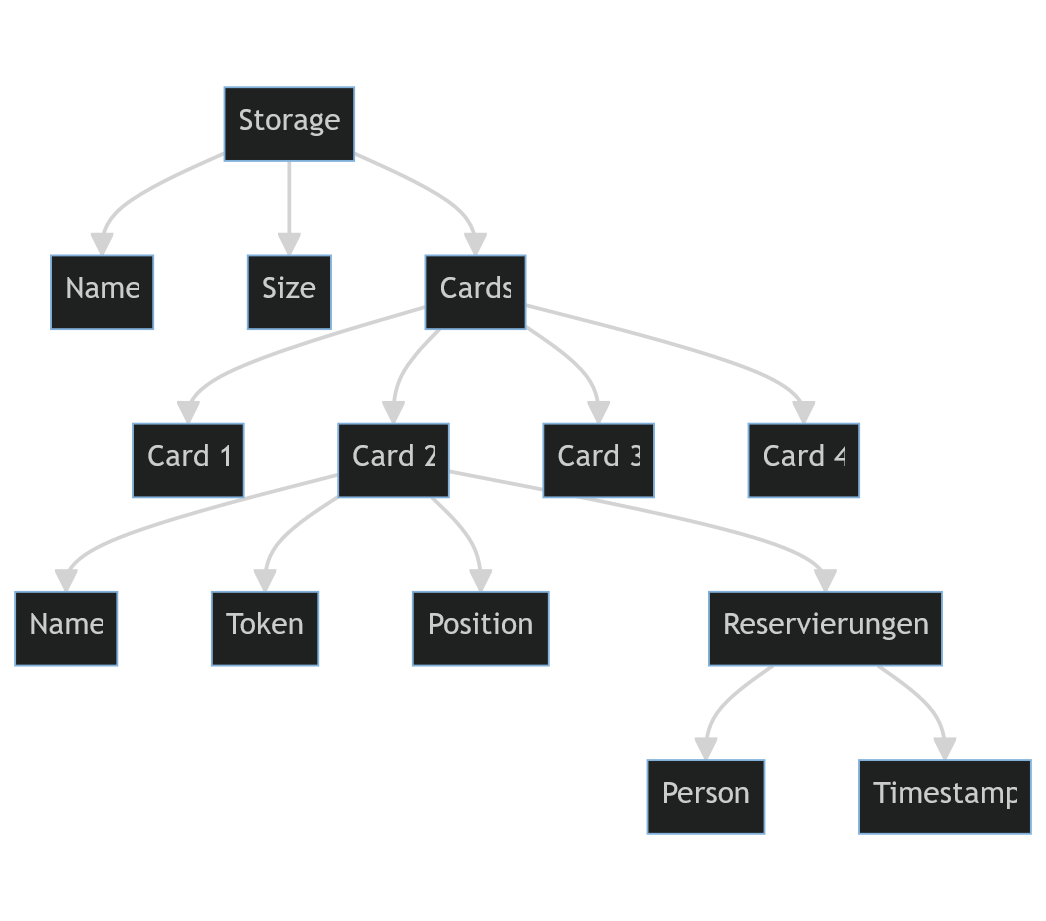
\includegraphics[width=1\textwidth]{FLUTTER/images/GP/JSON-Tree-Structur.png}
\caption{Beispiel einer JSON Baumstruktur mit mehreren \nameref{subsubsec:thero:dtos}}
\end{figure}

\newpage

\subsubsection{Data Transfer Objects}\label{subsubsec:thero:dtos}
Ein Data Transfer Object (DTO) beschreibt eine Entwurfsmuster-Klasse in der Softwareentwicklung, um Daten zwischen den verschiedenen Schichten einer Anwendung zu übertragen. Ein DTO beschreibt sozusagen einen Behälter für Daten, welcher von verschiedenen Komponenten der Applikation verwendet wird. \\
Meistens werden DTOs für die Speicherung von Daten, welche bei der Kommunikation zwischen eines Clients und Servers entstehen, verwendet. Diese werden im späteren Verlauf verarbeitet oder angezeigt. 

\begin{figure}[h!]
\centering
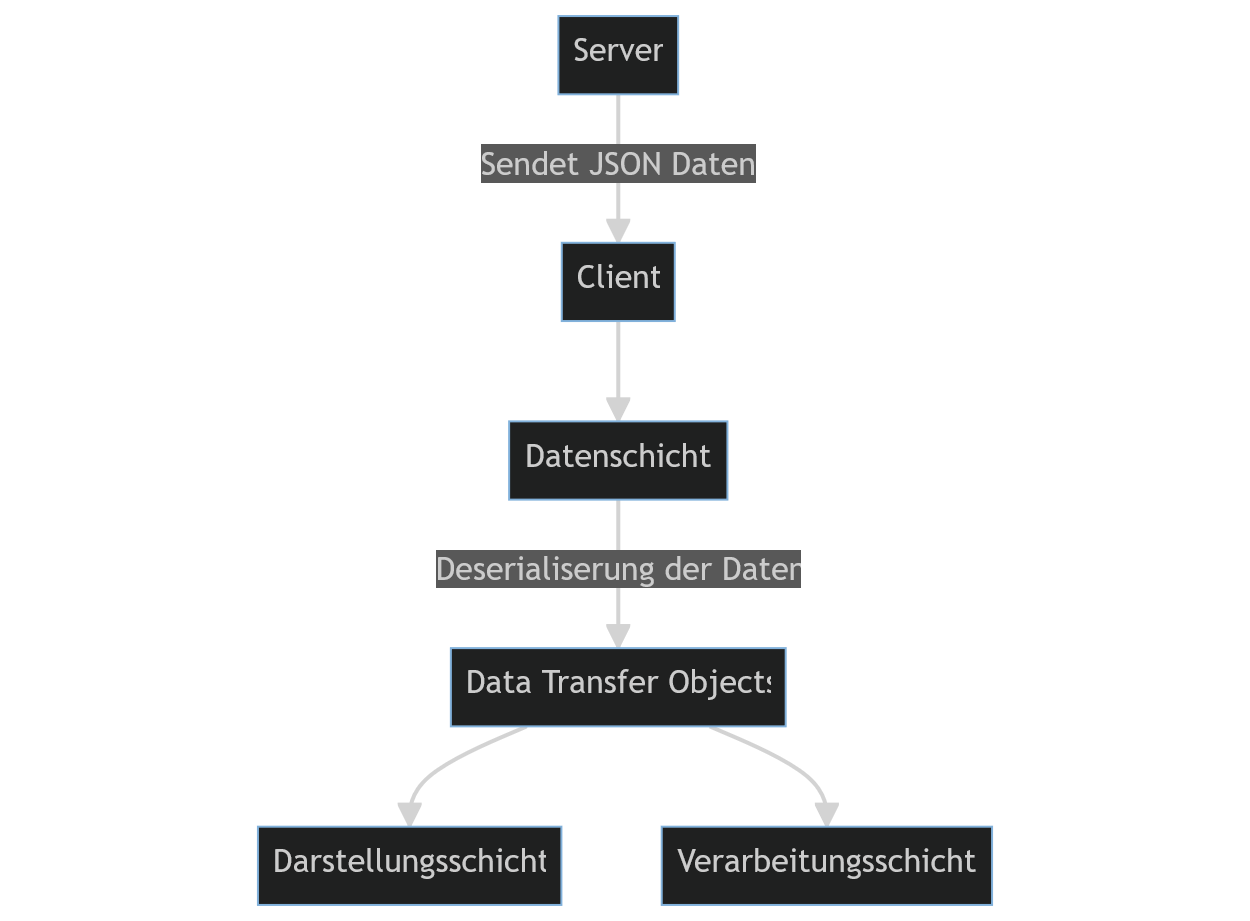
\includegraphics[width=0.7\textwidth]{FLUTTER/images/GP/deserialization.png}
\caption{Ablauf der Deserialisierung in Data Transfer Objects}
\end{figure}

Diese Grafik schildert den Ablauf der Deserialisierung der JSON Daten in DTOs.
\begin{itemize}
    \item Zunächst sendet der Server serialisierte Daten in Form einer JSON Struktur
    \item Die Informationen werden vom Client erhalten und innerhalb der Datenschicht in DTOs deserialisiert bzw. gespeichert.
    \item Die gespeicherten Daten können nun von der Darstellungs bzw. Verarbeitungsschicht verwendet werden. 
\end{itemize}

Die genaue Beschreibung der Architektur und Schichten erfolgt im Abschnitt \ref{sec:architecureflutter} \nameref{sec:architecureflutter} bzw. \ref{subsec:seperationlayers} \nameref{subsec:seperationlayers}

\newpage

\subsection{Responsive Design}\label{subsec:thero:responsive}
Unter einer responsiven Benutzeroberfläche wird die Eigenschaft verstanden, dass das Layout der App je nach Bildschirmgröße bzw. Bildschirmauflösung richtig angezeigt und skaliert wird. Das heißt, dass es egal ist, ob die App auf einem Tablet mit einem großen Bildschirm oder auf einem Smartphone mit einem kleinen Bildschirm angezeigt wird, da alles richtig formatiert wird. (vgl. \cite{responsive-design})

Grundsätzlich werden folgende Methoden angewendet, um ein Responsive Design bei der Programmierung mit Flutter umzusetzen:
\begin{itemize}
    \item {\textbf{Flüssiges Layout}}: Die Größe der Elemente einer Benutzeroberfläche wird anstelle von statischen Einheiten, bspw. Pixel, mit relativen Einheiten, bspw. Prozenten angegeben. Dadurch passt sich das Layout an verschiedene Bildschirmgrößen an.
    
    \item {\textbf{MediaQuery}}: Mittels des Media Query Widgets, können Daten wie Pixeldichte oder die Größe des Displays ermittelt werden. Durch diese Informationen ist es den Entwicklern möglich, das Layout dynamisch anzupassen
    
    \item {\textbf{Widget}}: Es gibt eine Vielzahl von Widgets, die bereits in der Flutter SDK enthalten sind, welche die Größe und das Verhalten der Widgets an das gegebene Layout anpassen.
\end{itemize}

Die Umsetzung des responsiven Designs wird im Abschnitt \ref{subsec:responsivedesign} \nameref{subsec:responsivedesign} behandelt

\begin{table}[htbp]
  \centering
  \begin{tabular}{cc}
    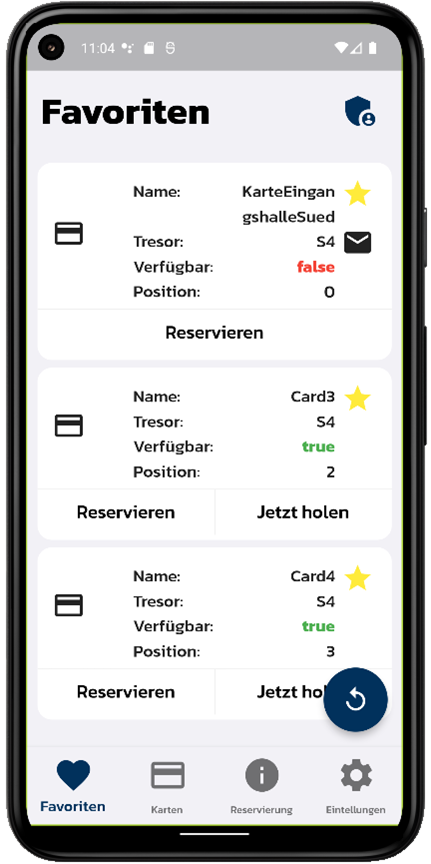
\includegraphics[width=0.15\textwidth]{FLUTTER/images/GP/Client_Karten.png} &
    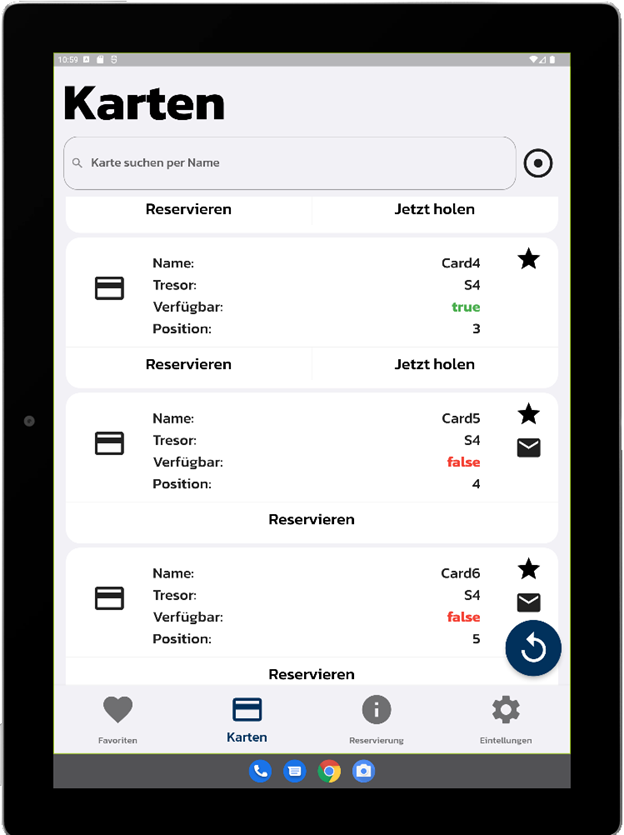
\includegraphics[width=0.25\textwidth]{FLUTTER/images/GP/client_responsive_tablet.png} \\
  \end{tabular}
  \label{tab:example}
  \captionsetup{type=figure}
\caption{Darstellung am Handy (links) und Tablet (rechts)}
\end{table}

\newpage

\section{Strukturierung der Anwendung}

\GpSSec{Login-Sicht }\label{subsec:thero:login}

\begin{wrapfigure}{r}{0.4\textwidth}
\centering
    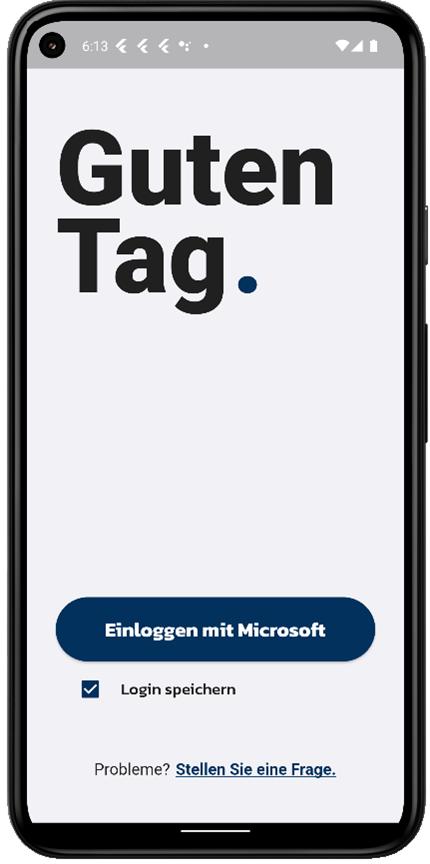
\includegraphics[width=0.25\textwidth]{FLUTTER/images/GP/Login_Allg.png}
    \caption{Login Anwendung}
\end{wrapfigure}




Die Login-Sicht stellt den Startbildschirm der Anwendung dar, auf dem sich der Benutzer mit seinem Microsoft-Konto anmelden und seine Registrierung abschließen kann. Bei erfolgreicher Registrierung wird der Benutzer zur Client-Anwendung weitergeleitet, wo er/sie Karten anfordern oder reservieren kann. 
\\
Um sich vollständig zu registrieren, muss die Karte einer Lehrkraft gescannt werden. Während des Anmeldevorgangs wird nach dem Standort bzw. Schlie\ss fach für den bevorstehenden Scan der Karte gefragt.\\

Falls Probleme während des Registrierungsvorgangs auftreten sollten, können Sie jederzeit den Support kontaktieren und eine Frage stellen. Zudem haben Sie die Möglichkeit, Ihre Anmeldedaten zu speichern.

Die genaue Beschreibung sowie Bedienung der Funktionalitäten erfolgt im Abschnitt \ref{sec:userguider:loginview}


\nameref{sec:userguider:loginview}

\newpage

\GpSSec{Client–Sicht }\label{subsec:thero:client}
\begin{wrapfigure}{r}{0.45\textwidth}
\centering
    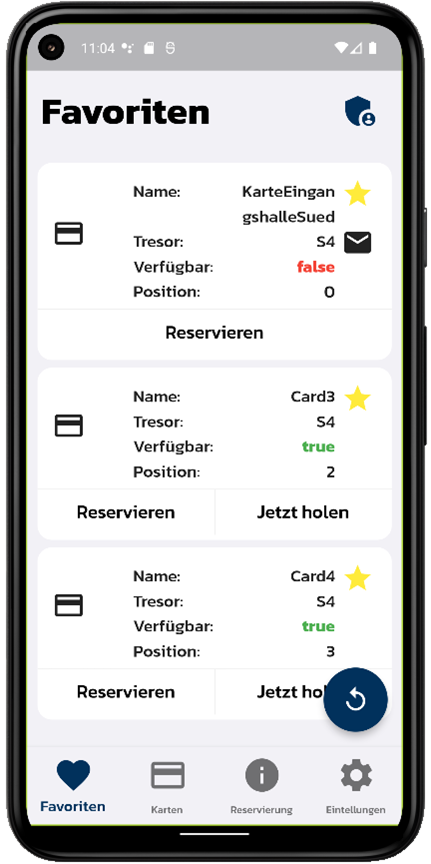
\includegraphics[width=0.25\textwidth]{FLUTTER/images/GP/Client_Karten.png}
    \caption{Client Sicht}
\end{wrapfigure}

Bei der Client Sicht handelt es sich um einen registrierten Benutzer, welcher durch die Bedienung der Benutzeroberfläche verschiedene Aktionen bspw. die Reservierung einer Karte durchführen kann. Der Ablauf der Registrierung wird im Abschnitt \ref{subsec:Registrierungsvorgang} \nameref{subsec:Registrierungsvorgang} behandelt. 
Die Hauptaufgabe der Client-Sicht ist es, die Karten, welche in den {\textit{Storages}} angelegt wurden, anzuzeigen und je nach Eigenschaft der Karten verschiedene Handlungen zu ermöglichen. Es wurde eine Navigation durch die Applikation erstellt, um eine übersichtlichere Aufteilung der einzelnen Aktionen zu ermöglichen.\\
Um auf die Admin-Anwendung zu wechseln, wird je nach Rechten bei der Kopfleiste ein Icon generiert, der bei Aktivierung auf die Administratoren Ansicht wechselt

\begin{itemize}
    \item Der Navigationsabschnitt \textbf{Karten} ermöglicht es, eine Karte anzufordern oder zu reservieren.

    \item Die \textbf{Favoriten-Seiten} zeigt alle favorisierten Karten an. Diese Seite hat die gleichen Eigenschaften wie die \textbf{Karten-Seite}.

    \item Unter \textbf{Reservierungen} werden alle reservierten und derzeit benutzten Karten angezeigt. Auf dieser Seite können Reservierungen gelöscht werden.

    \item Im Abschnitt \textbf{Einstellungen} werden verschiedene Optionen angeboten, wie z.B. das Einsehen der Account-Informationen, das Abmelden und weitere Einstellungsmöglichkeiten.
\end{itemize}
 Die genauere Beschreibung der Funkionalit\"aten und Bedienung ist im Abschnitt \ref{sec:userguider:clientview} aufzufinden.

\newpage
 
\ZbSSec{Admin – Sicht } \label{subsec:thero:admin}

Die Admin-Sicht ist als administrative Schnittstelle gedacht, bei der ausgewählte Lehrkräfte (Administratoren) Einstellungen am System vornehmen können. Diese Sicht kann aber nur von Benutzern benutzt werden, welche auch als Administratoren vermerkt sind. Die Admin-Sicht hat als Hauptaufgabe das Verwalten von Schließfächern, welche mit RFID Karten befüllt sind. Zu den Aufgaben zählen das Anlegen neuer Karten, das Bearbeiten von Karten und das Löschen von Karten. Des Weiteren können auch neue Schließfächer angelegt, bearbeitet und gelöscht werden. Weitere Funktionen sind, das Setzen von Administratoren und das Löschen von Benutzern und Reservierungen. Es gibt aber auch Funktionen zum Überwachen der Schließfächer. Dazu zählen das Pingen von Schließfächern, Statistiken zu den Karten anzuzeigen und Logs über das System als gesamtes anzeigen zu können. Alle dieser Funktionen werden im späteren Verlauf noch genauer beschrieben.\\
\\Um den Admin-Login verwenden zu können, muss ein Benutzer ein Administrator sein. Ein Benutzer kann Admin werden, indem ihn ein bereits existierender Admin in der Admin-Sicht unter Benutzer-Einstellungen zu einem Admin macht. Wenn dies getan wurde, steht dem Benutzer die Möglichkeit offen in die Admin-Sicht zukommen. Im gesamten System wird eine klare Trennung zwischen Admins und nicht Admins vorgenommen. Ein normaler Benutzer hätte nicht die Möglichkeiten wie ein Admin, auch wenn er sich als Admin anmelden könnte!\\
 \\ Die genauere Beschreibung der Funktionalitäten und Bedienung ist im Abschnitt \ref{sec:admin} aufzufinden.

\newpage

\begin{figure}[h!]
\centering
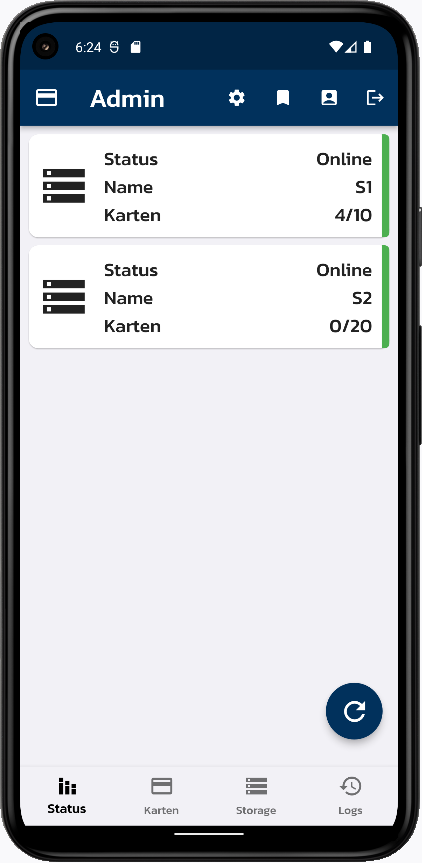
\includegraphics[width=0.3\textwidth]{FLUTTER/images/ZB/status_page.png}
\caption{Admin Sicht}
\end{figure}

\begin{itemize}
    \item Die \textbf{Status-Seite} ermöglicht es, einen kurzen Überblick über den aktuellen Status des Schließfach zu erhalten.
    \item Die \textbf{Karten-Seite} ermöglicht alles rund um Karten durchzuführen, Karten anlegen/bearbeiten und löschen.
    \item Die \textbf{Schließfach-Seite} ermöglicht alles rund um Schließfächer durchzuführen, Schließfächer anlegen/bearbeiten und löschen.
    \item Die \textbf{Log Seite} zeigt alle Transaktionen der API im Hintergrund an.
    \item Die \textbf{Reservierung-Seite} dient dazu, Reservierung zu löschen und die späteste Abholzeit der Karte einzustellen.
    \item Die \textbf{Benutzer-Seite} dient dazu, Benutzer zu einem Admin zu machen und Benutzer zu löschen.
    \item Die \textbf{Einstellung-Seite} wird zum Ändern des Themes und zu wechseln zur Client-Sicht verwendet.
\end{itemize}

\newpage

\GpSSec{Display-Sicht }\label{subsec:thero:display}
Die Display-Anwendung ist ebenfalls in Flutter programmiert und wird am Display des Schließfaches angezeigt. Sie dient, als visuelle Unterstützung sowie Möglichkeit Karten auszuleihen,
\begin{itemize}
    \item Auf der Navigationsseite ``Karten`` werden alle Karten des jeweiligen Schließfachs angezeigt. Registrierte Benutzer können hier eine Karte anfordern, indem sie ihre bei der Registrierung gespeicherte Kartennummer mit dem Kartenlesegerät am Schließfach scannen.
    \item Die Reservierung-Seite zeigt alle Reservierungen des jeweiligen Schließfachs an.
    
    \item Beim Scannen einer Karte erscheint ein Dialog am Bildschirm, der die restliche Zeit zum Scannen anzeigt.
    
    \item Nach jeder Aktion erscheint ein Feedback-Dialog, der je nach Erfolg bzw. Misserfolg eine Nachricht ausgibt.
\end{itemize}
    
Eine detaillierte Beschreibung und Anleitung zur Bedienung der Funktionalitäten findet sich im Abschnitt \ref{sec:userguider:displayview} \nameref{sec:userguider:displayview}

\begin{figure}[h!]
\centering
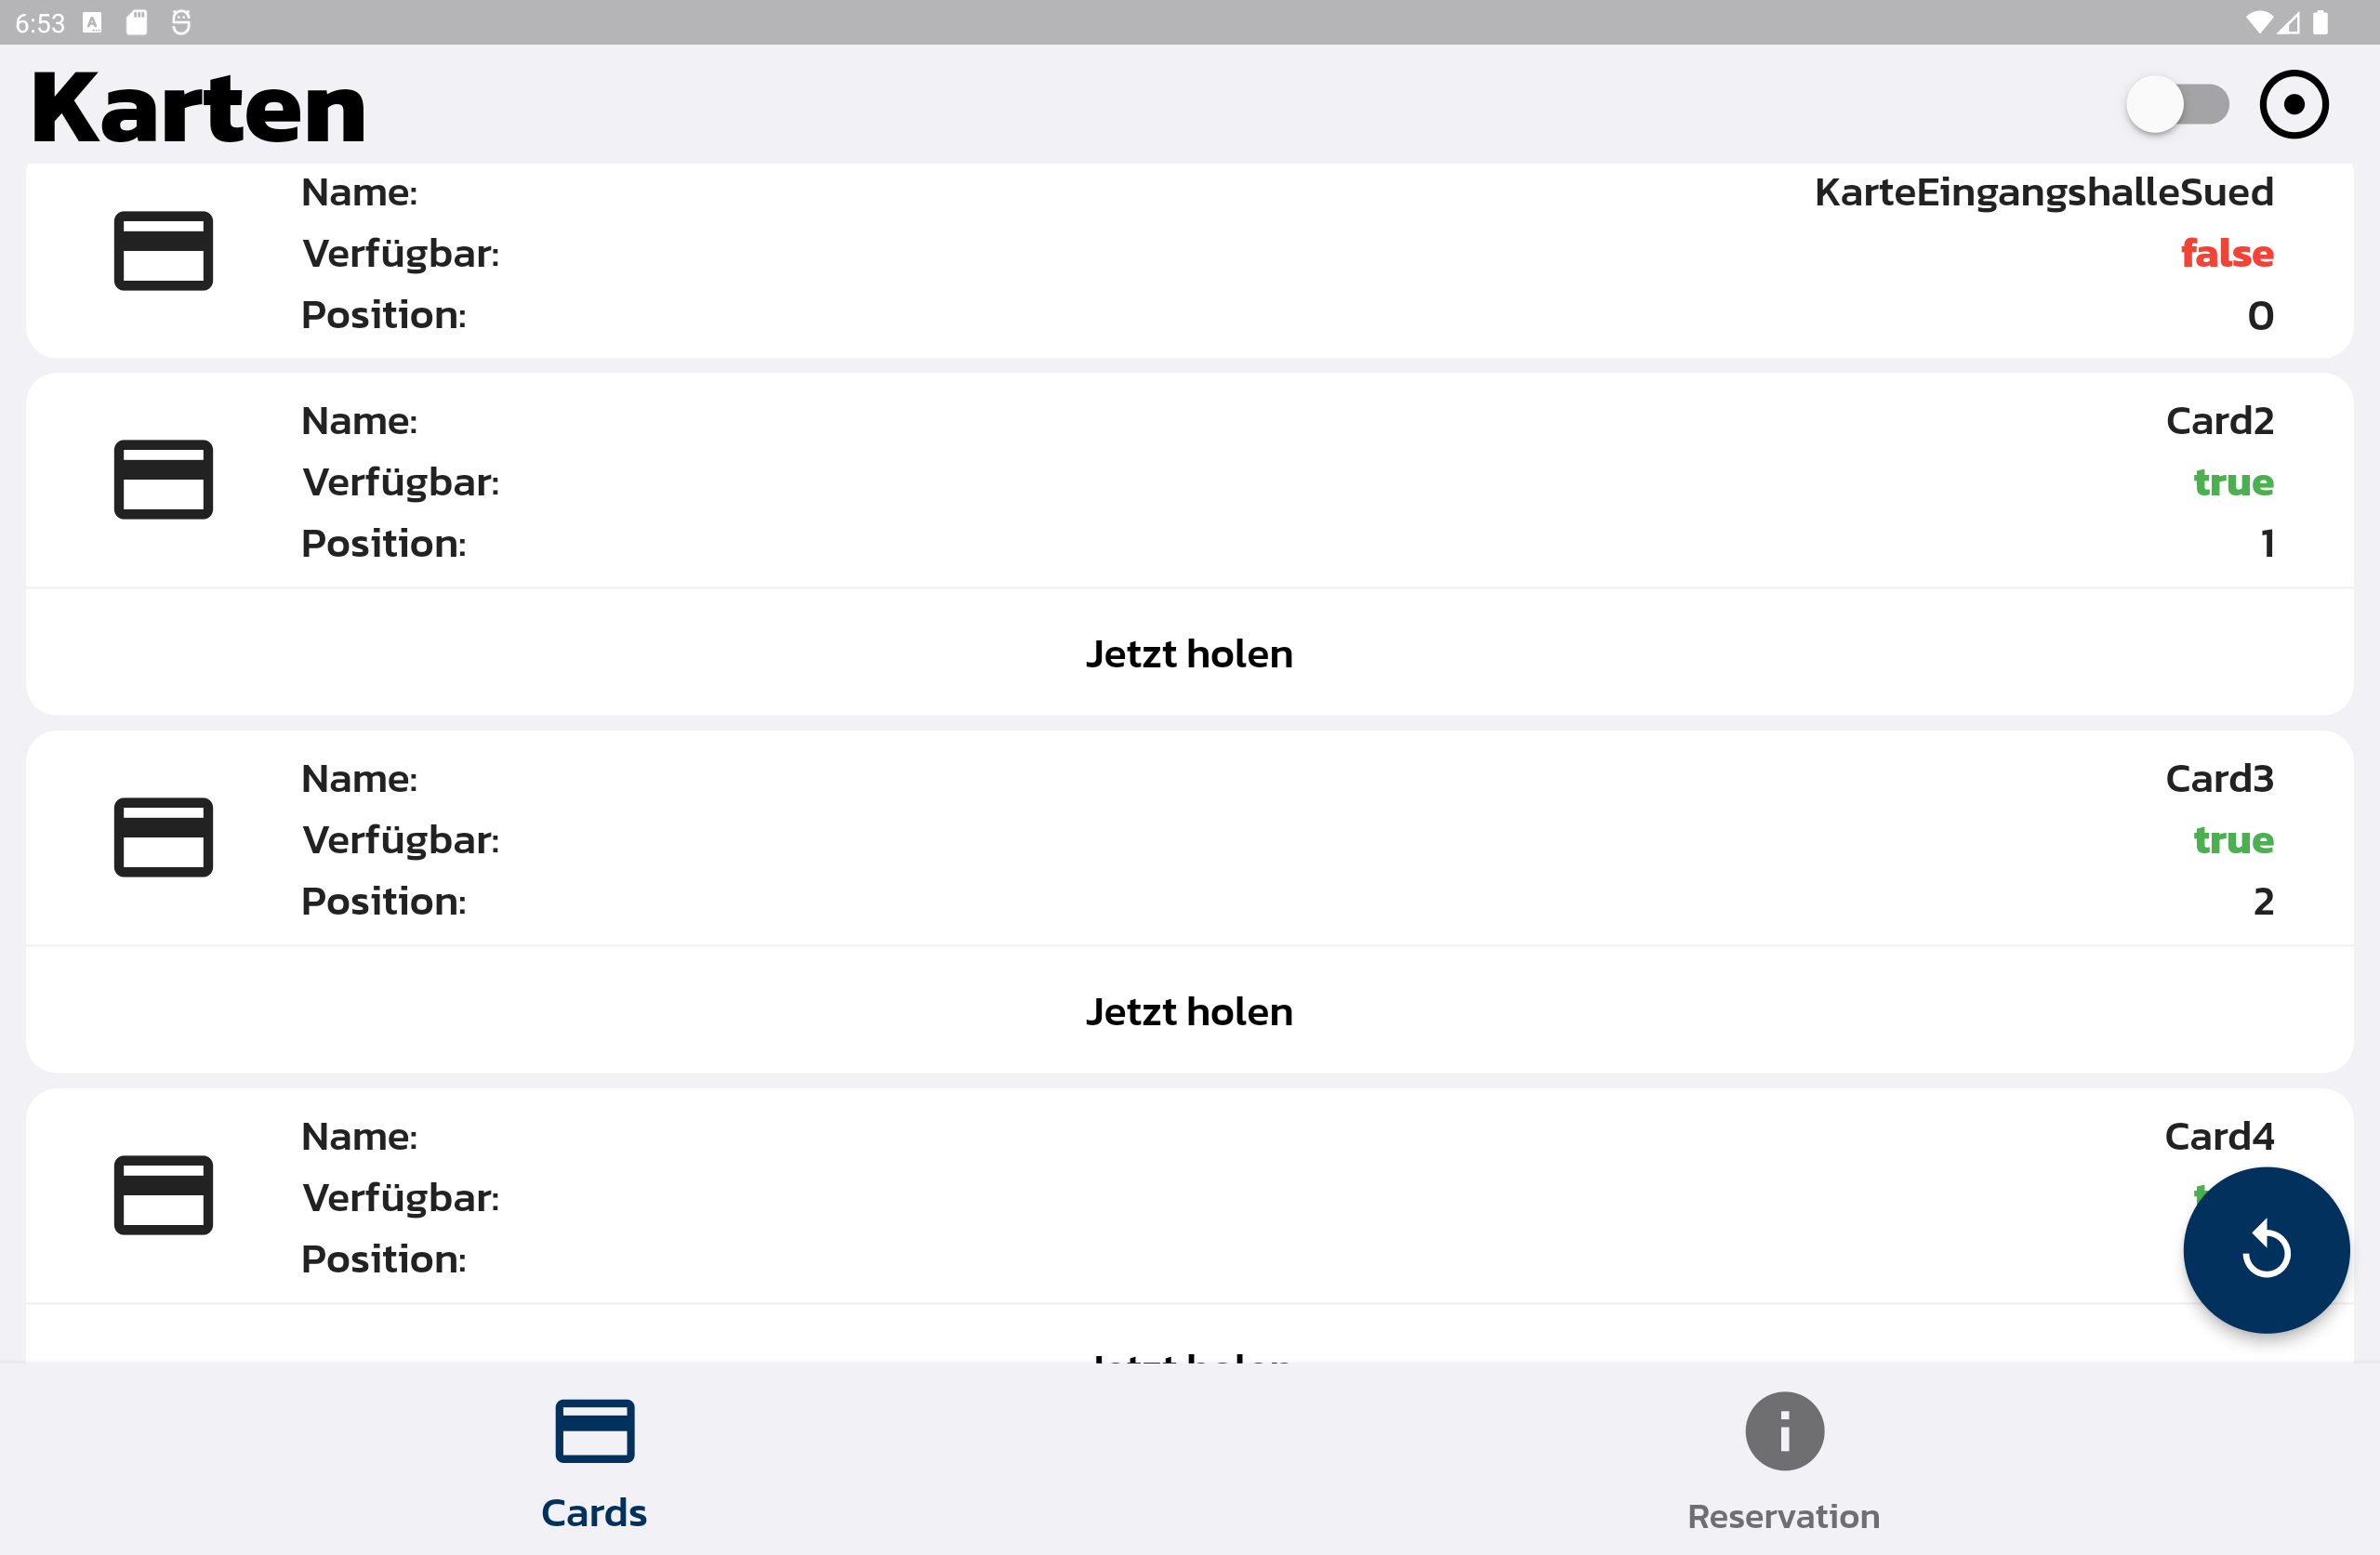
\includegraphics[width=0.75\textwidth]{FLUTTER/images/GP/Display_Allg.png}
\caption{Display Sicht}
\end{figure}

\newpage